% Tau and Muon Lifetime
% Project write up

\documentclass[aps,prl,groupedaddress]{revtex4}
\usepackage{graphicx}
\usepackage{amsmath}

\begin{document}

\title{Lepton Lifetime Experiment}
\author{Chris Martin}
\affiliation{Johns Hopkins University, Department of Physics and Astronomy}

\begin{abstract}
This document examines a hypothetical experiment to measure the lifetimes of various leptons. It outlines a computer program written in C++ using libraries included the the ROOT analysis package \cite{ROOT} and standard GNU utilities. The program simulates a beam of leptons ($e$, $\mu$, $\tau$)  incident on an ideal detector. After the events are generated the program uses a Log-likelihood fitting procedure in two different regimes $t < 1.0\cdot10^{-5} \mu s$ and $1.0\cdot10^{-5} \mu s < t < 50 \mu s$ to determine the $\tau$ and $\mu$ lifetimes respectively. 

\end{abstract}

\maketitle

\section{Monte Carlo}
\subsection{Beam and Detector}
Here we discuss the assumed limitations of the detector. The beam of leptons is assumed to be a gaussian distribution peaked at 1000 MeV with a standard deviation of 10MeV. Each particle generated is assigned a random energy weighted by the specified gaussian distribution. Every time the program is run it generates this distribution again and the output is stored in $Beam\_Energy.png$ shown in Figure \ref{fig:BeamE}. Each particle has its observed lifetime dilated by an amount calculated from its mass and its assigned energy. The beam is assumed to allow each particle to enter the detector individually so that all events can be studied. 

\begin{figure}[htp]
\centering
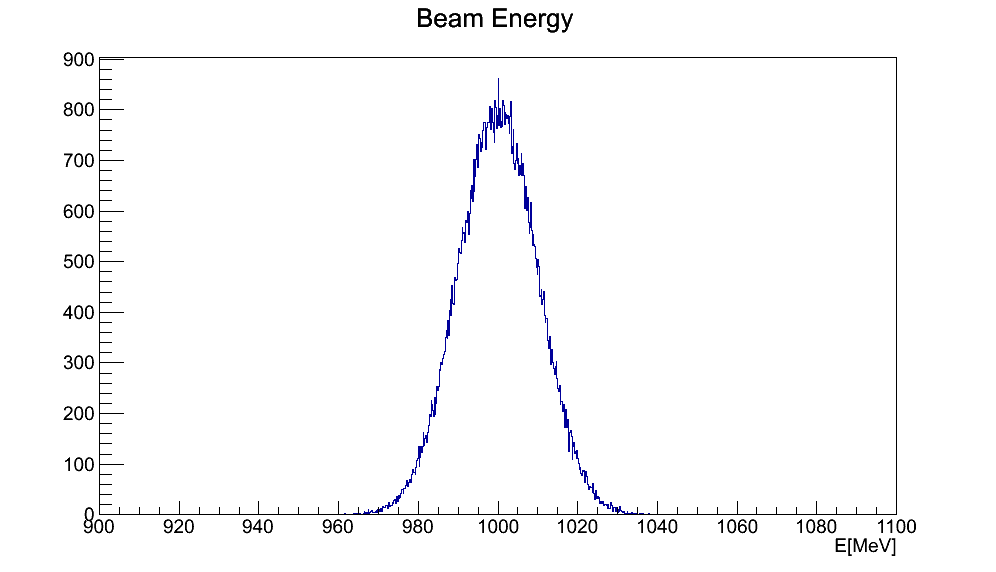
\includegraphics[height=100mm]{Beam_Energy.png}
\caption{Distribution of Beam Energies}
\label{fig:BeamE}
\end{figure}

The detector is assumed to see only the decay of a particle. It is assumed to have "infinite" time resolution so that the very short lifetime of the $\tau$ lepton can be studied. To provide a limit on how long the detector will wait for a particle to decay an arbitrary limit $t_{max} = 50 \mu s$ is set on the detector.

\subsection{Lepton Generation}
The first part of the Project generates 100000 possible events. Each event is first assigned a flavor. Each flavor has equal weight and has the accepted values for the mass, lifetime, and the respective errors in these values. These values are taken from the PDG and can be found in table \ref{tab:Prop} or in \cite{PDG}.


\begin{table}[ht]
\caption{Lepton Properties}
\begin{tabular}{| c | c | c | c |}
\hline
  & Electron & Muon $(\mu)$ & Tau $(\tau)$ \\
 \hline
Mass & $0.510998910 \pm 0.000000013$ MeV & $105.658367 \pm 0.000004$ MeV & $1776.82 \pm 0.16$ MeV \\
\hline
Lifetime & $> 4.6 \cdot 10^{26}$ yr &  $(2.197034 \pm 0.000021) \cdot 10^{-6}$ s & $(290.6 \pm 1.0) \cdot 10^{-15}$ s \\
\hline
\end{tabular}
\label{tab:Prop}
\end{table}

The properties for the electron are ignored because the lifetime is much longer than I wish to run the simulation. So the electron is assumed to have an infinite lifetime and thus will not decay within the hypothetical detector. The Probability Density Function for a particle decaying at a time $t$ is given by the Exponential distribution \ref{eq:Expo}. Where $\tau$ is the lifetime of the flavor given by \ref{tab:Prop}.

\begin{equation}
\label{eq:Expo}
P(t;\tau) = \frac{e^{\frac{-t}{\tau}}}{\tau}
\end{equation}

From this expression one can obtain integrate to obtain an expression for the set of random times $t_{i}$ in \ref{eq:t_i}. Where $r_{i}$ is a random number between 0 and 1. 

\begin{equation}
\label{eq:t_i}
t_{i} = -\tau \cdot log(1-r)
\end{equation}

As explained in the previous section these times are stretched due to the relativistic effects of the $1000$ MeV beam. If this time becomes longer than $50 \mu s$ it is assumed that the detector will timeout and no signal will be recorded.

\section{Likelihood Fit}
\subsection{Binning}
After the events are generated they are divided into two categories $t < 1.0\cdot10^{-5} \mu s$ and $1.0\cdot10^{-5} \mu s < t < 50 \mu s$. Each category is divided into 100 bins and the number of decays in each bin is plotted on a log scale using the standard Histogram class in ROOT. The output is stored in $Tau\_MC.png$ and $Muon\_MC.png$.

\subsection{Log-Likelihood}
The Likelihood function for N events is the product of the individual probability functions given by \ref{eq:like}. The object is to find the value of $\tau$ that maximizes this likelihood.

\begin{equation}
\label{eq:like}
\mathcal{L} = \prod P(t;\tau) = \prod \frac{e^{\frac{-t}{\tau}}}{\tau}
\end{equation}

Because the probabilities are always less than 1 we will maximize the log-likelihood so that the numbers don't get too small for the computer to handle. Thus solving the equation \ref{eq:LogLike} will give the best value of the lifetime.

\begin{equation}
\label{eq:LogLike}
\frac{d}{d \tau} ln[\mathcal{L}] = \frac{d}{d \tau} \left\{ \frac{-1}{\tau} \sum t - N \cdot ln[\tau] \right\} = 0
\end{equation}

\subsection{ROOT Fit}
The program uses the ROOT standard Log-Likelihood fit and the standard TMath libraries. Each time regime is fit with a function of the form:

\makebox[\textwidth]{[0]*TMath::Exp(-t/[1])}\par

The results of the fit can be found in the graphs \ref{fig:Tau} and \ref{fig:Muon}.

\begin{figure}[htp]
\centering
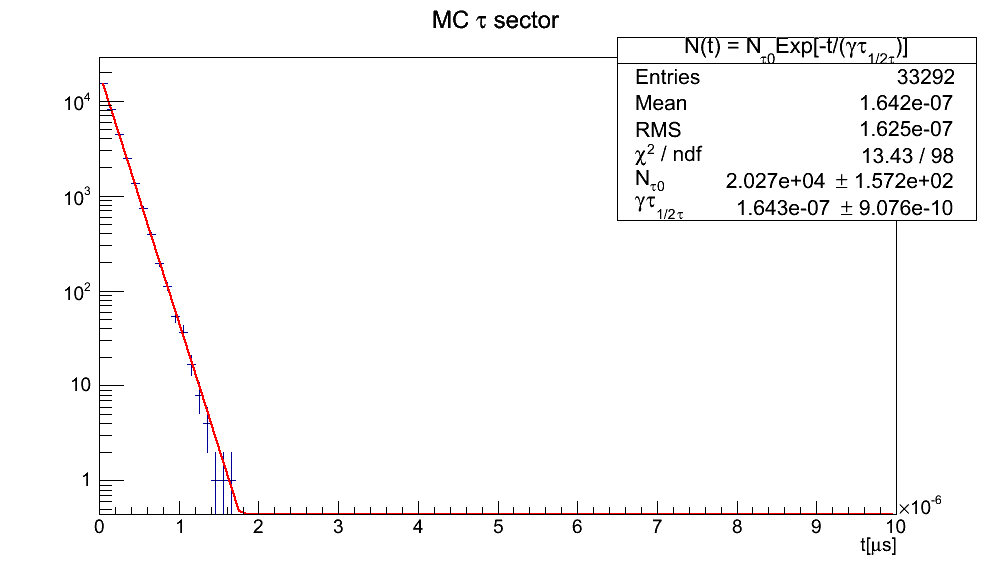
\includegraphics[height=100mm]{Tau_MC.png}
\caption{$\tau$ Likelihood fit}
\label{fig:Tau}
\end{figure}

\begin{figure}[htp]
\centering
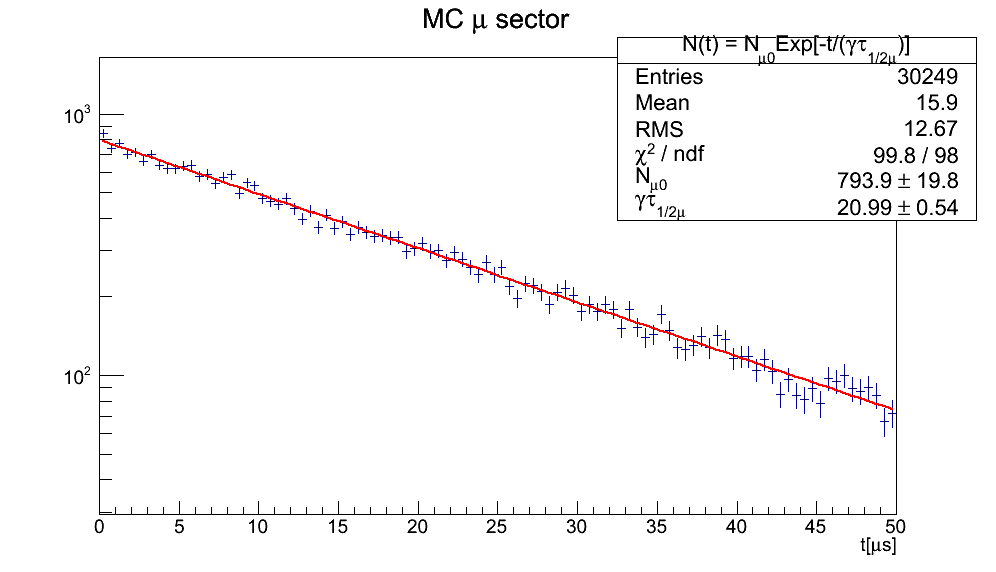
\includegraphics[height=100mm]{Muon_MC.png}
\caption{$\mu$ Likelihood fit}
\label{fig:Muon}
\end{figure}

\section{Results}
The results of the fit give acceptable agreement between the accepted values and the ones generated by the MC generation and fit procedure. The experiment found values of 
$2.21768 \pm 0.0612643 \mu s$ and $2.9186 \cdot 10^{-07} \pm 3.33456 \cdot 10^{-09} \mu s$ for the Muon and Tau Lepton lifetimes.  These show reasonable agreement with the accepted values found in Table \ref{tab:Prop}.
\begin{thebibliography}{2}

\bibitem{ROOT}
\emph{ROOT; a data analysis framework}, CERN, Version 5.20.00

\bibitem{PDG}
\emph{The Review of Particle Physics}, K. Nakamura et al. (Particle Data Group), J. Phys. G 37, 075021 (2010) and 2011 partial update for the 2012 edition.

\end{thebibliography}

\section{Code}
\subsection{$makefile$}

\subsection{$Project.cpp$}

\subsection{$Lifetime.cpp$}

\subsection{$Lifetime.h$}

\section{Output files}
\subsection{$Likelihood\_output.txt$}

\subsection{$Project-ChrisMartin.txt$}

\subsection{$Tau\_MC.png$}

\subsection{$Muon\_MC.png$}

\subsection{$Beam\_Energy.png$}

\end{document}
